\section{Results}
\label{sec:results}

Figure~\ref{fig:flow} is a placeholder image under \texttt{figures/}. Drop binary
assets (images, data dumps) into \texttt{assets/}, put generation or
post-processing helpers in \texttt{scripts/}, and keep scratch notes or drafts
in \texttt{misc/}.

\begin{figure}[ht]
  \centering
  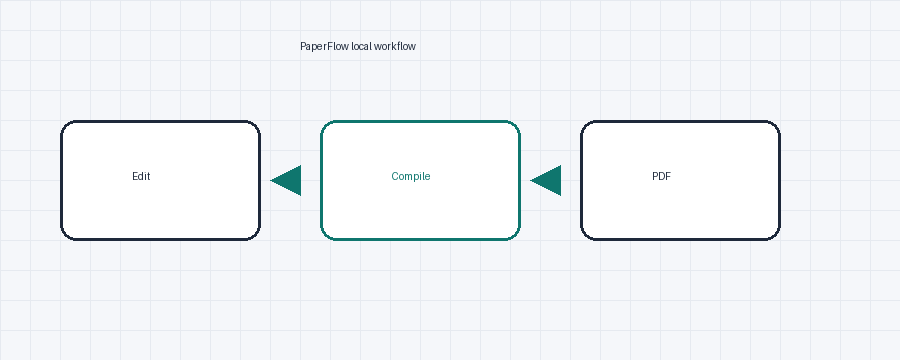
\includegraphics[width=0.72\linewidth]{figures/flow.png}
  \caption{Example figure loaded from the project tree.}
  \label{fig:flow}
\end{figure}

Metrics for this demo: \MetricFigureCount{} figure and \MetricSectionCount{} sections
(\MetricWordCount{} words of fluff).
